\newsection
\subsection{Language}
\label{sec:language}
\sectionauthors{Isabel Papadimitriou, Christopher D. Manning}

\subsubsection{The nature of human language}

Language is the basis of most human communication and interaction. However, it is not just a means for humans to achieve shared goals: language is central to human thought, to how social and emotional relations are formed, to how we identify ourselves socially and personally, and to how humans record knowledge and develop societal intelligence.
Spoken or signed languages arise in every human society, and the languages of the world are both incredibly diverse in the ways that they express and structure the information they convey, while also exhibiting surprising concordance in the richness of what makes a language \citep{comrie1989language}.
Languages are remarkably complex yet efficient systems, acquired consistently by children in a short amount of time, and which evolve and encompass the changing needs and conditions of linguistic communities. 
Due to this centrality of language in human activities, language understanding and generation is a critical element of research in artificial intelligence. 
Natural language processing (NLP) is the subfield of artificial intelligence concerned with language and, together with the related fields of automatic speech recognition (ASR) and text-to-speech (TTS), has the goal of giving computers the ability to understand and generate human language in much the same way human beings can. 

To date in 2021, NLP has been the field most profoundly affected by foundation models. The first generation of foundation models showcased an impressive variety of linguistic abilities, as well as a surprising amount of adaptability to a large range of linguistic situations. Since the introduction of the early foundation models ELMo \cite{peters2018elmo} and BERT \cite{devlin2019bert} in 2018, the field of NLP has become largely centered around using and understanding foundation models.
The field has shifted to using foundation models as the primary tool, moving towards more generalized language learning as a central approach and goal. 
In this section, we go over the recent successes of foundation models in NLP, detail how foundation models have changed the overall process and mentality for training machine learning models for language, and discuss some of the theoretical and practical challenges facing foundation models as they are being applied to a broader set of languages and more realistic and complex linguistic situations.

 \begin{figure}[t]
\centering
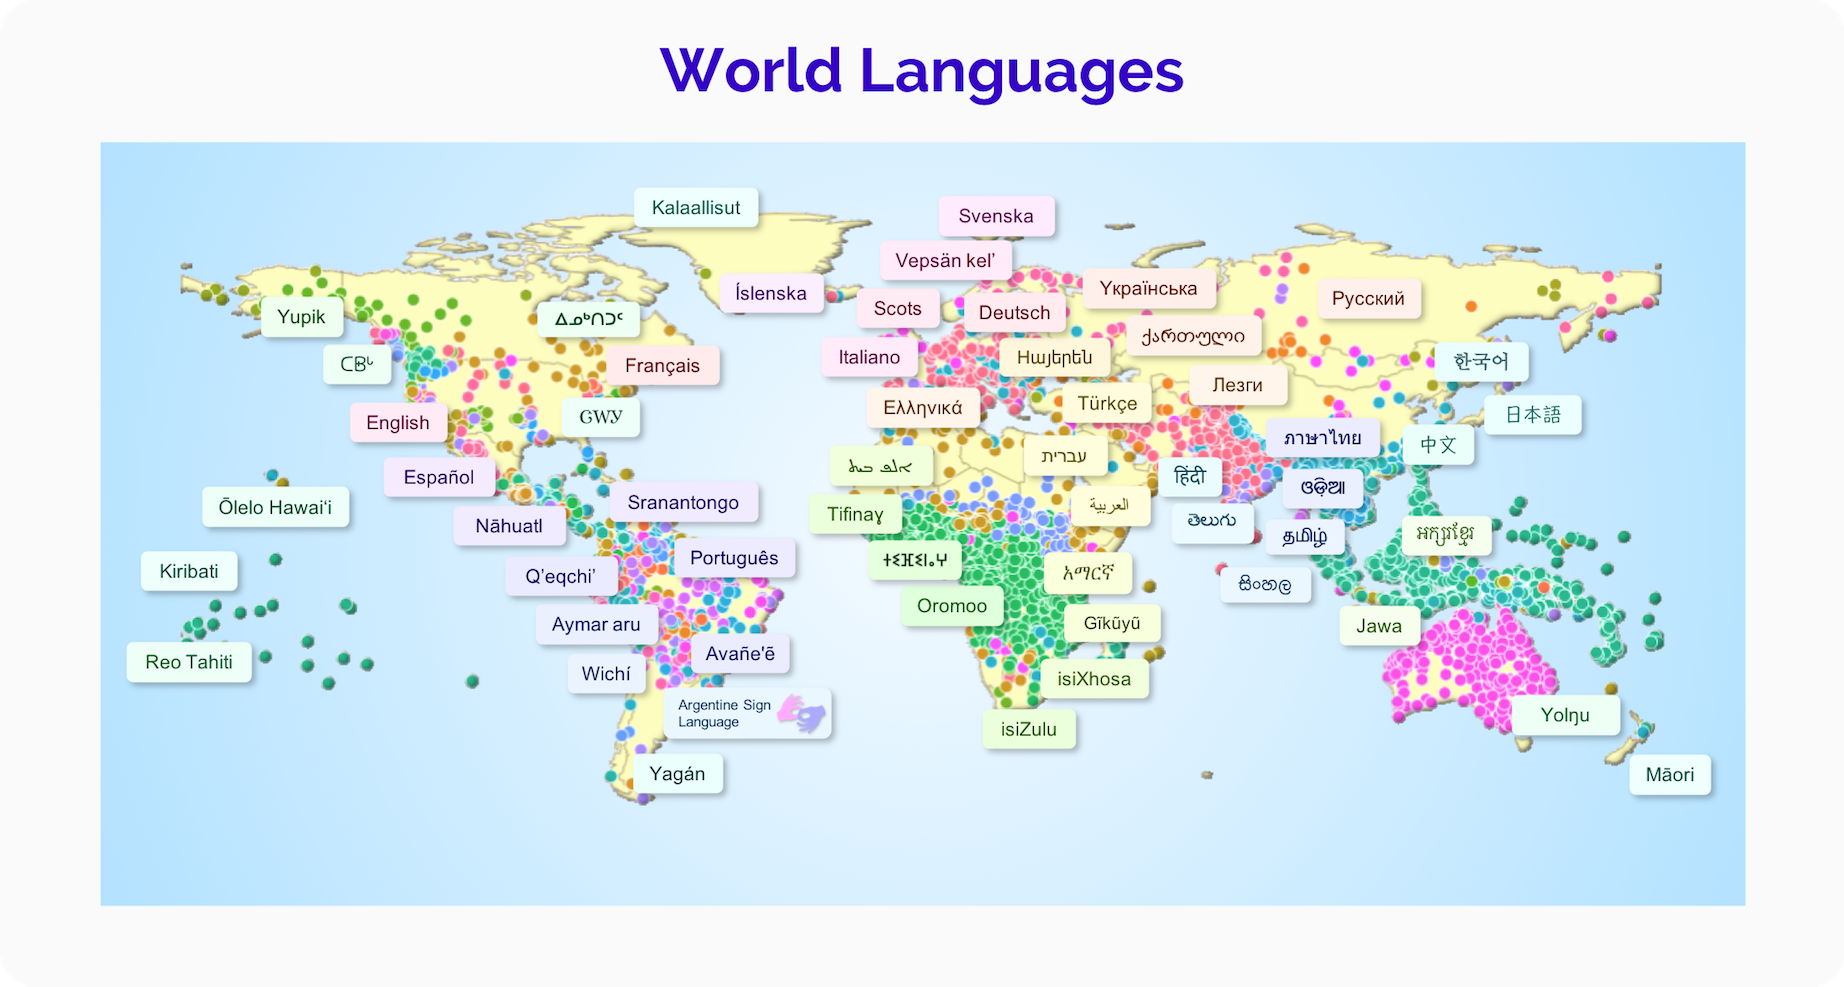
\includegraphics[width=\textwidth]{capabilities/figures/Language_1.png}
\caption{\label{fig:language_1}
There are over 6,000 languages in the world, though estimates vary due to the inherent uncertainty of what constitutes a separate language \citep{nordhoff2011glottolog}. This map shows the languages of the world, with each dot representing one language and color indicating the top-level language family for each language. Data is from Glottolog \cite{glottolog}. We label a few of the languages on the map as examples. Only a tiny percentage of the world's languages are currently represented in foundation models.}
\end{figure}

\subsubsection{Impact of foundation models on NLP}

Foundation models have had a huge impact on the field of NLP, and are now central to most NLP systems and research. On a first level, many foundation models are skilled language generators: for example, \citet{clark2021all} demonstrate that non-experts have difficulty distinguishing short-form English text that was written by GPT-3 from that written by humans. However, the feature of foundation models that has been most impactful in NLP is not their raw generation abilities but their surprising \textit{generality and adaptability}: a single foundation model can be adapted in different ways in order to solve many linguistic tasks.  

The field of NLP has historically focused on creating and solving challenging linguistic tasks, with the vision that building models that solve these tasks will lead to competent language systems for downstream applications.  NLP tasks include \textit{classification tasks} for a whole sentence or document (\eg sentiment classification, like predicting  whether a movie review is positive or negative), \textit{sequence labeling} tasks, in which we classify each word or phrase in a sentence or document  (\eg predicting if each word is a verb or a noun, or which spans of words refer to a person or an organization),  \textit{span relation classification}, (\eg relation extraction or parsing, like whether  a person and location are linked by a ``current residence'' relation, or a verb and a noun by a ``subject-verb'' relation) and \textit{generation tasks}, producing new text that is conditioned strongly on an input (\eg producing a translation or summary of a text, recognizing or producing speech, or responding in a conversation) 
\citep{jurafsky2009speech}.
In the past, NLP tasks had distinct research communities that developed task-specific architectures, often based on pipelines of different models, each performing a linguistic sub-task such as token segmentation, syntactic parsing, or coreference resolution.

By contrast, the dominant modern approach for performing each task is to use a single foundation model and adapt it slightly using relatively small amounts of annotated data specific to each task (sentiment classification, named entity tagging, translation, summarization) to create an adapted model (see \refsec{adaptation} for a detailed view of adaptation).
This has proved to be an extremely successful approach: for the vast majority of the tasks described above, a foundation model that is slightly adapted for a task greatly outperforms previous models or pipelines of models that were built specifically to solve that one task. To take just one example, the best system for answering open-ended science questions in 2018, before foundation models, could get 73.1\% on the NY Regents 8th grade science exam. A year later in 2019, an adapted foundation model scored 91.6\% \citep{clark2019aristo}.

The emergence of foundation models that are largely trained to \textit{generate} language has constituted an important shift in the role of language generation in NLP. 
Until around 2018, the problem of generating general-purpose language was considered very difficult and
essentially unapproachable except through other linguistic sub-tasks \citep{paris2013natural}.
Instead,  NLP research was mostly focused on linguistically analyzing and understanding text. 
Now, it is possible to train highly coherent foundation models with a simple language generation objective, like ``predict the next word in this sentence''. These generative models now constitute the primary vehicle through which machine learning for language is done\dash{}including the analysis and understanding tasks that were once considered prerequisites for generation. 
The successful generation exhibited by foundation models has also led to a flowering of research for language generation tasks like summarization and dialogue generation. 
The rise of the foundation model paradigm has begun to play a similar role in spoken language as well as written.  Modern automatic speech recognition (ASR) models like wav2vec 2.0 are trained on large datasets of speech audio alone, and then adapted on audio with associated transcriptions for the task of ASR \citep{wav2vec2}.

Due to the changes brought about by the foundation model paradigm, the focus of research and practice in NLP has shifted from making bespoke architectures for different tasks to exploring how to best leverage foundation models. Research into adaptation methods has blossomed 
(see \refsec{adaptation} for a detailed look at adaptation), and the surprising successes of foundation models have also caused a shift in research interest towards analyzing and understanding foundation models
(see \refsec{interpretability} for interpretability and analysis of foundation models).

\subsubsection{Language variation and multilinguality}

Though foundation models are surprisingly versatile with the linguistic knowledge they obtain from pretraining,
there are limits to this adaptability: it is not clear how successfully current foundation models handle language variation.
Language varies greatly. Apart from the fact that there are thousands of different languages in the world, language varies even within one language or within one speaker. To point out a few examples, informal conversation manifests differently from written language, the grammatical constructions that people reach for when speaking to friends are very different from those used when speaking to someone with authority, and communities of speakers within a language use different dialects. Social and political factors are embedded in how language variation is viewed and valued, and in how much different varieties are represented in NLP research (see for example \citet{blodgett17} on the failures of NLP for African American English, and \refsec{fairness} for a deeper discussion on inequities in foundation models).
Due to their large capacity for learning linguistic information and flexibly adapting that knowledge, foundation models hold promise for expanding NLP to encompass more linguistic diversity. It remains an open research question to understand whether it is possible to make foundation models that robustly and equitably represent language with both its major and subtle variations, giving equal weight and acuity to what makes each linguistic variety distinct \citep[research posing and addressing this question includes][]{ponti2019modeling, bender2011achieving, joshi2020state}.

Following the success of foundation models in English, multilingual foundation models have been released to extend that success to non-English languages.
For most of the over 6,000 languages in the world, the text data available is not enough to train a large-scale foundation model with. 
To give one example, there are over 65 million speakers of Fula, a West African language, but few if any resources available for NLP in Fula \citep{nguer2020sencorpus}.
Multilingual foundation models address this by jointly training on multiple languages at the same time, and the multilingual foundation models to date (mBERT, mT5, XLM-R) are each trained on around 100 languages \citep{devlin2019bert, goyal2021larger, xue2020mt5}. Joint multilingual training relies on the reasonable assumption that the shared structures and patterns between languages can lead to sharing and transfer from the high-resource languages to the low-resource ones, making foundation models possible for languages where we could not train a stand-alone model.
Experiments using and analyzing multilingual foundation models have shown that there is indeed a surprising amount of transfer between and parallel encoding of the different languages in multilingual foundation models \citep{wu-dredze-2019-beto, choenni2020cross, pires2019multilingual, libovicky2019language, chi2020finding, papadimitriou2021deep, cao2019multilingual}.  

However, the extent to which these models are robustly multilingual is still an open question. 
It remains unclear how much models trained on this data can represent aspects of other languages that are drastically different from English, or if their apparent multilingual performance relies more on assimilation \citep{lauscher2020zero, virtanen2019multilingual, artetxe_cross-lingual_2020}. Multilingual models show better performance in languages that are similar to the highest-resource languages in their training data, and it has been shown that languages in multilingual models compete for model parameters, making it unclear how much variation can fit in a single model \citep{wang2020negative}. A salient issue stems from the data that we use to train multilingual foundation models: in many multilingual corpora, English data is not only orders of magnitude more abundant than that of lower-resource languages, but it is often cleaner, broader, and contains examples showcasing more linguistic depth and complexity \citep{caswell2021} (see \citet{nekoto2020participatory} on building participatory and robust multilingual datasets).
However, the answer does not simply lie in creating more balanced corpora: there are so many axes of language variation that it would be infeasible to create a corpus that is balanced and representative in all regards. The future, versatility, and equity of foundation models all depend on robustly handling language variation despite unbalanced data \cite[\eg][]{oren2019drolm}.

Current multilingual foundation models in their raw form, and naive unsupervised multilingual training as a method, may not deeply model the subtleties of languages and language varieties to their full extent. Nevertheless, they remain useful for some multilingual applications, for example through adapting multilingual models for low-resource languages not in their original training set \citep{wang2020extending}.
The research community should critically examine how foundation models deal with language variation, understand the limits of foundation models in bringing equity and representation to NLP, and not settle on promoting foundation models that erase language variation and mostly conform to the linguistic majority in their training data. 

\subsubsection{Inspiration from human language acquisition}

\begin{figure}[t]
\centering
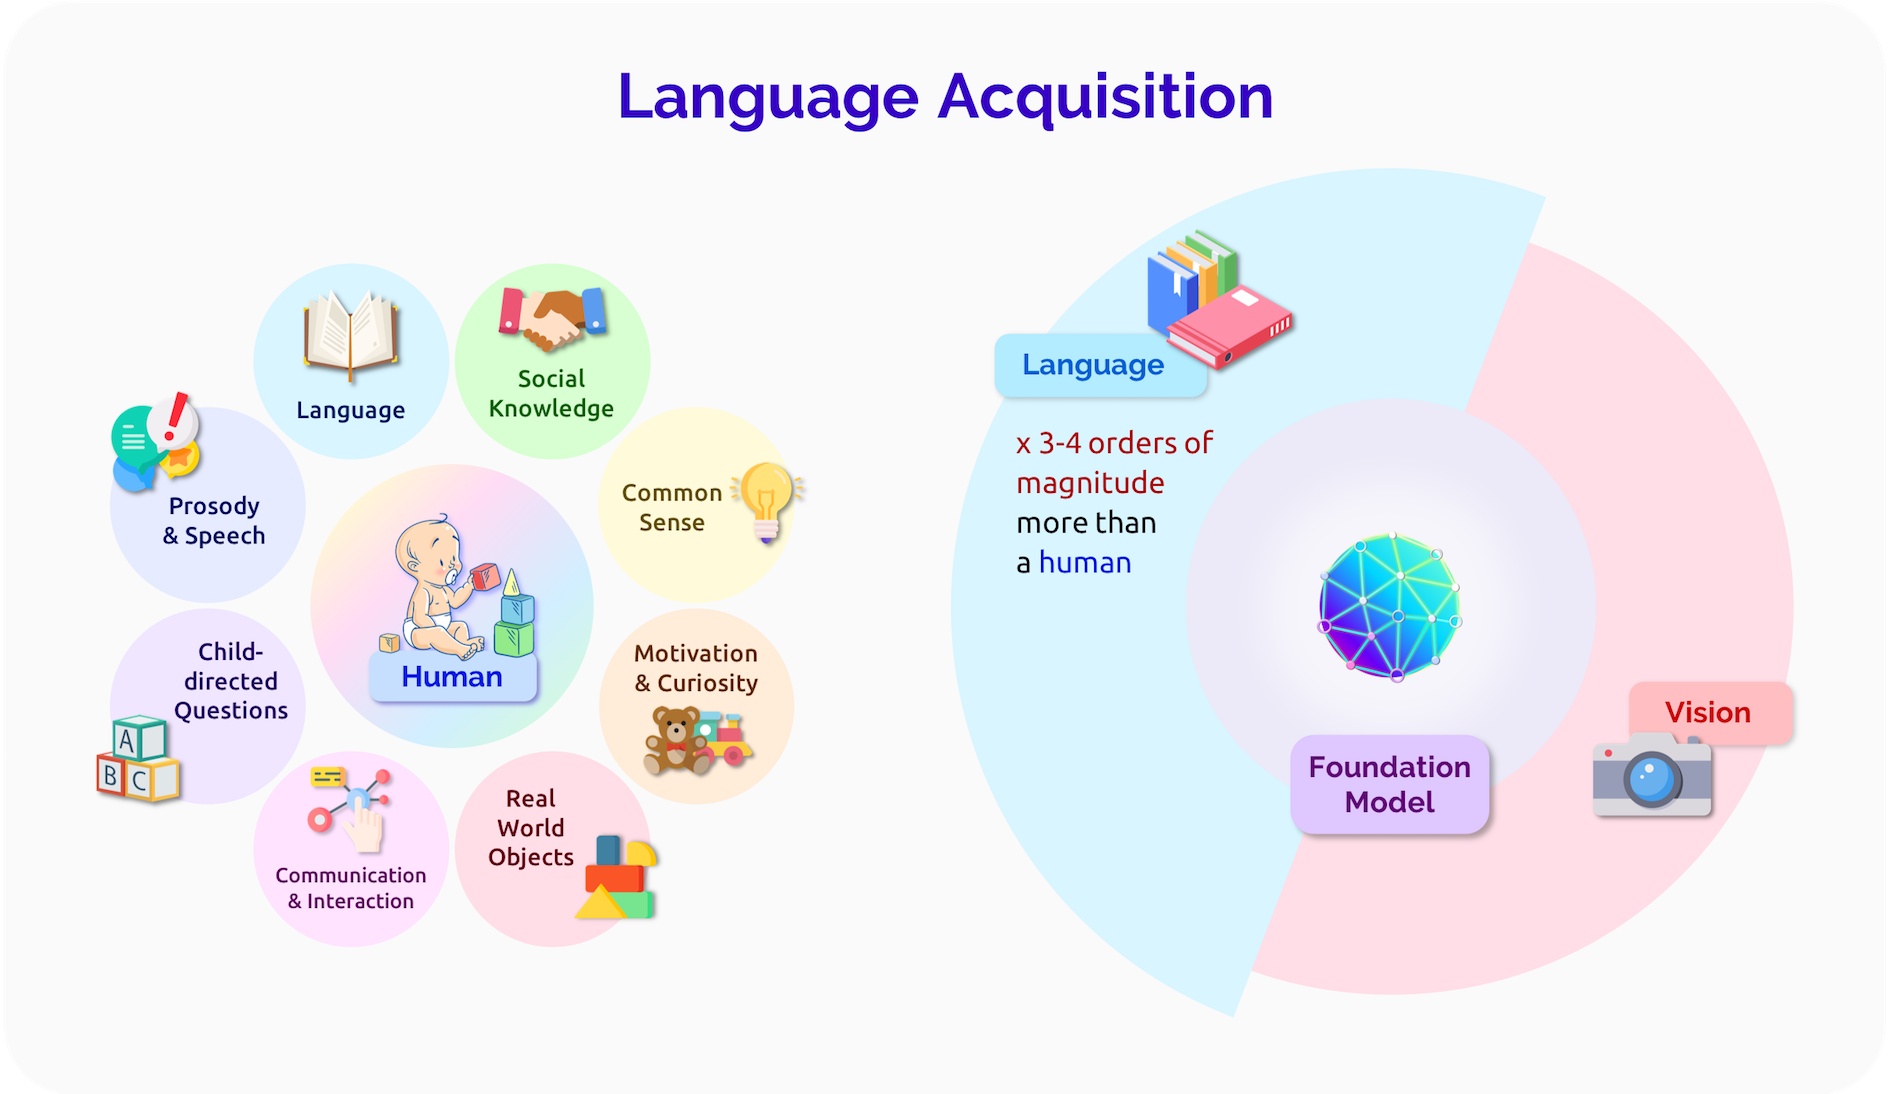
\includegraphics[width=\textwidth]{capabilities/figures/Language_2.png}
\caption{\label{fig:language_2}
Language Acquisition for humans and foundation models. While there are certainly different inductive biases between the human brain and foundation models, the ways that they learn language is also very different. Most saliently, humans interact with a physical and social world in which they have varied needs and desires, while foundation models mostly observe and model data produced by others.}
\end{figure}

Though foundation models have constituted a huge source of progress in creating NLP systems that act more like humans, there are still significant ways in which the linguistic system that they acquire, as well as the learning process, differ from human language. Understanding the implications of this gap between machine and human language learning is a necessary part of developing a research community informed about the linguistic limits and possibilities of foundation models.

Human language acquisition is very efficient: foundation models like GPT-3 are trained on around three to four orders of magnitude more language data than most humans will ever hear or read, and certainly much more than children have been exposed to by the time they are mostly linguistically competent. 
One salient difference between foundation models and human language acquisition is that human language is grounded to the real world. 
For example babies and caretakers point to objects during language development \citep{colonnesi2010relation}, and babies learn the grounded meanings of words that refer to common objects before they learn a lot of the other aspects of the linguistic system \citep{bergelson20126}. Most foundation models used in NLP, on the other hand, learn from the distributional information of raw, ungrounded text, and (in contrast to human learners) \citet{zhang2021billions} show that RoBERTa models express abstract syntactic features before usable meaning. Powerful ungrounded statistical learning is indeed also present in babies \citep{saffran1996statistical}, so it is no doubt an important factor in acquisition. Nevertheless, advancing grounded language learning for foundation models remains an important direction for approaching human acquisition efficiency
\citep[\textit{inter alia}]{dupoux2018cognitive, tan2020vokenization, zellers2021piglet} (see \refsec{vision} and \refsec{robotics} for the multimodal potential of foundation models, and \refsec{philosophy} for a discussion of whether foundation models can understand language without grounding). 
Another important direction is examining the inductive biases in foundation models and how they relate to the inductive biases in the human mind, both those specific to language learning and those general to human cognition \citep{linzen2021syntactic}. Though the human brain may be more architecturally specialized for efficient language acquisition, foundation models are not blank-slate learners \cite{baroni2021proper}, and understanding and aligning these linguistic inductive biases is an important future direction for research in foundation models. 

A significant factor in the efficiency of language acquisition is the fact that humans acquire a systematic and generalizable language system. Though there are many differing theories about what types of theoretical abstractions the human language system makes \citep[\eg][]{comrie1989language, chomsky2014minimalist, croft2001radical, jackendoff2011human}, it is generally agreed that humans learn language in a way that allows them to easily slot new knowledge into existing abstractions, and productively create new grammatical sentences. For example, a ten-year-old child has acquired a lot of the abstractions about how their language works, though the actual words and constructions that they produce will change drastically over the next ten years. Foundation models, on the other hand, often do not acquire the systematic abstractions that we expect from humans. For example, when a foundation model produces a linguistic construction accurately one time there is no guarantee
that future uses of that construction will be mostly consistent, especially after a significant domain shift in the subject matter \citep[examples of work examining limitations of foundation models in systematicity include][]{lake2018generalization, kim2020cogs, bahdanau2018systematic, chaabouni2021can}. NLP faces the challenge of developing some sort of systematicity in acquisition for foundation models, without regressing to systems that rely too heavily on rigid linguistic rules.

Language learning continues for a speaker's whole lifetime:
the grammar of human languages evolves, and humans flexibly adapt to novel linguistic situations \citep{sankoff2018change}. For example, as new terms and concepts arise in an adult's life they can use them relatively easily in grammatical sentences, and humans often adapt their grammatical patterns to fit in with different social groups \citep{rickford1994addressee}. 
On the other hand, the linguistic system of foundation models is mostly set by the training data, and is relatively static \citep{lazaridou2021pitfalls, Khandelwal2020Generalization}. Though adaptation methods can prime foundation models for different tasks (see \refsec{adaptation}), it still remains unclear how to change the more basic linguistic foundation of a foundation model without a large amount of training. 
Making adaptable models that naturally mirror human-like linguistic accommodation and language evolution is an important research area for the future of foundation models.

Foundation models have drastically changed research and the practice of NLP.
Most of the complex NLP tasks that the research community focused on solving before foundation models, are now best solved to an almost-human level using one of a few publicly-released foundation models. Yet, there remains a gap between this performance and the immediate and safe usefulness of foundation models in complex downstream settings. Foundation models have also given rise to many new research directions for the community: understanding generation as a fundamental aspect of language, studying how to best use and understand foundation models, understanding the ways in which foundation models may increase inequities in NLP,  examining whether foundation models can satisfactorily encompass linguistic variation and diversity, and finding ways to draw on human language learning dynamics. 